\chapter{Algebra di Boole: assiomi, proprietà e sintesi}
\label{ch:boole-sintesi}
\textit{(13 marzo -- 16 marzo 2026)}

\section{Tempi caratteristici delle porte logiche}

\begin{definizione}{Tempo di propagazione}
\textbf{Tempo di propagazione} $t_P$: calcolato fra $V_{in}$ e $V_{out}$; è il tempo che intercorre fra i momenti in cui i segnali raggiungono il 50\% della loro intensità fra $V_{OL}$ e $V_{OH}$. È dovuto alle risposte dei transistor (inter-sat).

\medskip
\textbf{Tempo di transizione} $t_r$: si misura su un \emph{solo} segnale ($V_{in}$ oppure $V_{out}$); è il tempo fra i momenti in cui il segnale è al 10\% e al 90\% della sua escursione (salita) o al 90\% e al 10\% (discesa). È dovuto ad effetti capacitivi.
\end{definizione}

\section{Assiomi dell'algebra di Boole}

L'algebra di Boole è definita dai seguenti assiomi su un insieme $B$ con $|B|=2$:

\begin{itemize}[leftmargin=1.5em]
    \item \textbf{Chiusura}: $\forall\,a,b\in B \Rightarrow a+b\in B$ (OR) e $a\cdot b\in B$ (AND).
    \item \textbf{Elementi neutri}: $a+0=a$ \quad (0 è neutro per OR); \quad $a\cdot 1=a$ \quad (1 è neutro per AND).
    \item \textbf{Operazioni complemento}: $\overline{a}+a=1$ \quad e \quad $\overline{a}\cdot a=0$ \quad (elemento opposto).
    \item \textbf{Involuzione}: $\overline{\overline{a}}=a$.
\end{itemize}

\section{Proprietà dell'algebra di Boole}

\begin{itemize}[leftmargin=1.5em]
    \item \textbf{Commutativa}: $a+b=b+a$ \quad ; \quad $a\cdot b=b\cdot a$.
    \item \textbf{Associativa}: $(a+b)+c=a+(b+c)=a+b+c$ \quad ; \quad $(a\cdot b)\cdot c=a\cdot(b\cdot c)=a\cdot b\cdot c$.
    \item \textbf{Distributiva}: $(a+b)\cdot c=a\cdot c+b\cdot c$ \quad ; \quad $(a\cdot b)+c=(a+c)\cdot(b+c)$. \\
    \textit{Si verifica con le tabelle di verità.}
    \item \textbf{Dualità}: posso sempre scambiare un'operazione con l'altra insieme a tutti gli elementi (operazione, neutro, opposto). Funziona perché è un'algebra a 2 elementi, quindi 0 è uno e 1 è l'altro: $a+0=a \Rightarrow a\cdot 1=a$.
    \item \textbf{Assorbimento}: $a+a\cdot b=a$ \quad ; \quad (duale) $a\cdot(a+b)=a$.
    \item \textbf{Idempotenza}: $a+a=a$ \quad ; \quad $a\cdot a=a$.
\end{itemize}

\subsection{Teorema della semplificazione}

\[
x\cdot y + x\cdot\overline{y} = x
\]
\[
x\cdot y + x\cdot\overline{y} = x\cdot(y+\overline{y}) = x\cdot 1 = x
\]

\noindent\textit{Duale}: $(x+y)\cdot(x+\overline{y})=x$. Ad esempio, scambiando il ruolo delle variabili:
\[
(x+y)\cdot(\overline{x}+y)=x\overline{x}+xy+\overline{x}y+y=0+y\,(x+\overline{x})+y=y+y=y
\]

\subsection{Teorema della moltiplicazione e fattorizzazione}

\[
(x+y)\cdot(\overline{x}+z)=x\cdot z+\overline{x}\cdot y
\]

Dimostrazione:
\[
(x+y)\cdot(\overline{x}+z)=\overline{x}\cdot x+x\cdot z+\overline{x}\cdot y+y\cdot z
=x\cdot z+\overline{x}\cdot y+yz(x+\overline{x})
=x\cdot z(1+y)+\overline{x}\cdot y(1+z)=x\cdot z+\overline{x}\cdot y
\]
\textit{(usando $1+y=1$ per ogni $y$, e $yz=yz\,(x+\overline{x})$)}

\noindent\textit{Duale}: $(\overline{x}\cdot z)+(x\cdot y)=(\overline{x}+y)\cdot(x+z)$.

\subsection{Leggi di De Morgan}
\label{sec:demorgan}

\[
x+y+z+\cdots = \overline{\overline{x}\cdot\overline{y}\cdot\overline{z}\cdots}
\]
\[
x\cdot y\cdot z\cdots = \overline{\overline{x}+\overline{y}+\overline{z}+\cdots}
\]

% ======================================================================
\section{Porte universali: NAND e NOR}

Le porte NAND e NOR sono dette \textbf{porte universali} (o un set funzionalmente completo) perché con ciascuna di esse è possibile realizzare \emph{qualsiasi} funzione booleana, replicando il comportamento di NOT, AND e OR. 
Al contrario, AND e OR \emph{non} formano insiemi universali da soli, poiché, non potendo invertire un segnale, non permettono di realizzare la funzione NOT.

\subsection{NAND come porta universale}

\begin{fitcenter}
\begin{circuitikz}[scale=0.7, every node/.style={scale=0.7}]

% ---- NOT con NAND ----
\node[font=\small\bfseries, anchor=east] at (-1.0, 7.0) {NOT};
\node[nand port] (NN) at (1.5, 7.0) {};
\draw (NN.in 1) -- (NN.in 2);
\draw ($(NN.in 1)!0.5!(NN.in 2)$) -- ++(-0.8,0) node[left]{$A$};
\draw (NN.out) -- ++(0.5,0) node[right]{$\overline{A}$};

% ---- AND con NAND ----
\node[font=\small\bfseries, anchor=east] at (-1.0, 5.0) {AND};
\node[nand port] (NA1) at (1.5, 5.0) {};
\node[nand port] (NA2) at (3.5, 5.0) {};
\draw (NA1.in 1) -- ++(-0.8,0) node[left]{$A$};
\draw (NA1.in 2) -- ++(-0.8,0) node[left]{$B$};
\draw (NA2.in 1) -- (NA2.in 2);
\draw (NA1.out) -- ($(NA2.in 1)!0.5!(NA2.in 2)$);
\draw (NA2.out) -- ++(0.5,0) node[right]{$A \cdot B$};

% ---- OR con NAND ----
\node[font=\small\bfseries, anchor=east] at (-1.0, 3.0) {OR};
\node[nand port] (NO1) at (1.5, 3.5) {};
\node[nand port] (NO2) at (1.5, 2.5) {};
\node[nand port] (NO3) at (3.5, 3.0) {};
\draw (NO1.in 1) -- (NO1.in 2);
\draw ($(NO1.in 1)!0.5!(NO1.in 2)$) -- ++(-0.8,0) node[left]{$A$};
\draw (NO2.in 1) -- (NO2.in 2);
\draw ($(NO2.in 1)!0.5!(NO2.in 2)$) -- ++(-0.8,0) node[left]{$B$};
\draw (NO1.out) -- ++(0.3,0) |- (NO3.in 1);
\draw (NO2.out) -- ++(0.3,0) |- (NO3.in 2);
\draw (NO3.out) -- ++(0.5,0) node[right]{$A + B$};

% ---- XOR con NAND ----
\node[font=\small\bfseries, anchor=east] at (6.0, 7.0) {XOR};
\node[nand port] (NX0) at (8.0, 5.0) {};
\node[nand port] (NX1) at (9.8, 5.9) {};
\node[nand port] (NX2) at (9.8, 4.1) {};
\node[nand port] (NX3) at (11.6, 5.0) {};

% Inputs A and B (robustly drawn to the left)
\draw (NX1.in 1) -- ++(-2.7, 0) coordinate (Ain) node[left] {$A$};
\draw (NX2.in 2) -- ++(-2.7, 0) coordinate (Bin) node[left] {$B$};

% Taps to NX0
\path (Ain) -- (NX1.in 1) coordinate[pos=0.15] (tapA);
\path (Bin) -- (NX2.in 2) coordinate[pos=0.25] (tapB);
\draw (tapA) to[short, *-] (tapA |- NX0.in 1) -- (NX0.in 1);
\draw (tapB) to[short, *-] (tapB |- NX0.in 2) -- (NX0.in 2);

% Middle connections
\draw (NX0.out) -- ++(0.2,0) coordinate (NX0out_split);
\draw (NX0out_split) |- (NX1.in 2);
\draw (NX0out_split) |- (NX2.in 1);

% Final connections
\draw (NX1.out) -- ++(0.2,0) |- (NX3.in 1);
\draw (NX2.out) -- ++(0.2,0) |- (NX3.in 2);
\draw (NX3.out) -- ++(0.5,0) node[right]{$A \oplus B$};

\end{circuitikz}
\end{fitcenter}

\subsection{NOR come porta universale}

In modo duale alla NAND, anche la NOR può realizzare NOT, AND, OR e XOR:

\begin{fitcenter}
\begin{circuitikz}[scale=0.7, every node/.style={scale=0.7}]

% ---- NOT con NOR ----
\node[font=\small\bfseries, anchor=east] at (-1.0, 7.0) {NOT};
\node[nor port] (RN) at (1.5, 7.0) {};
\draw (RN.in 1) -- (RN.in 2);
\draw ($(RN.in 1)!0.5!(RN.in 2)$) -- ++(-0.8,0) node[left]{$A$};
\draw (RN.out) -- ++(0.5,0) node[right]{$\overline{A}$};

% ---- OR con NOR ----
\node[font=\small\bfseries, anchor=east] at (-1.0, 5.0) {OR};
\node[nor port] (RO1) at (1.5, 5.0) {};
\node[nor port] (RO2) at (3.5, 5.0) {};
\draw (RO1.in 1) -- ++(-0.8,0) node[left]{$A$};
\draw (RO1.in 2) -- ++(-0.8,0) node[left]{$B$};
\draw (RO2.in 1) -- (RO2.in 2);
\draw (RO1.out) -- ($(RO2.in 1)!0.5!(RO2.in 2)$);
\draw (RO2.out) -- ++(0.5,0) node[right]{$A + B$};

% ---- AND con NOR ----
\node[font=\small\bfseries, anchor=east] at (-1.0, 3.0) {AND};
\node[nor port] (RA1) at (1.5, 3.5) {};
\node[nor port] (RA2) at (1.5, 2.5) {};
\node[nor port] (RA3) at (3.5, 3.0) {};
\draw (RA1.in 1) -- (RA1.in 2);
\draw ($(RA1.in 1)!0.5!(RA1.in 2)$) -- ++(-0.8,0) node[left]{$A$};
\draw (RA2.in 1) -- (RA2.in 2);
\draw ($(RA2.in 1)!0.5!(RA2.in 2)$) -- ++(-0.8,0) node[left]{$B$};
\draw (RA1.out) -- ++(0.3,0) |- (RA3.in 1);
\draw (RA2.out) -- ++(0.3,0) |- (RA3.in 2);
\draw (RA3.out) -- ++(0.5,0) node[right]{$A \cdot B$};

% ---- XOR con NOR: 4 NOR danno lo XNOR, una quinta NOR (come NOT) lo nega ----
\node[font=\small\bfseries, anchor=east] at (6.0, 7.0) {XOR};
\node[nor port] (RX0) at (8.0, 5.0) {};
\node[nor port] (RX1) at (9.8, 5.9) {};
\node[nor port] (RX2) at (9.8, 4.1) {};
\node[nor port] (RX3) at (11.6, 5.0) {};
\node[nor port] (RX4) at (13.4, 5.0) {};
\draw (RX1.in 1) -- ++(-2.7, 0) coordinate (Ain) node[left] {$A$};
\draw (RX2.in 2) -- ++(-2.7, 0) coordinate (Bin) node[left] {$B$};
\path (Ain) -- (RX1.in 1) coordinate[pos=0.15] (tapA);
\path (Bin) -- (RX2.in 2) coordinate[pos=0.25] (tapB);
\draw (tapA) to[short, *-] (tapA |- RX0.in 1) -- (RX0.in 1);
\draw (tapB) to[short, *-] (tapB |- RX0.in 2) -- (RX0.in 2);
\draw (RX0.out) -- ++(0.2,0) coordinate (RX0split);
\draw (RX0split) |- (RX1.in 2);
\draw (RX0split) |- (RX2.in 1);
\draw (RX1.out) -- ++(0.2,0) |- (RX3.in 1);
\draw (RX2.out) -- ++(0.2,0) |- (RX3.in 2);
\draw (RX4.in 1) -- (RX4.in 2);
\draw (RX3.out) -- ($(RX4.in 1)!0.5!(RX4.in 2)$);
\node[above, font=\scriptsize] at ($(RX3.out)+(0.35,0.05)$) {XNOR};
\draw (RX4.out) -- ++(0.4,0) node[right]{$A \oplus B$};

\end{circuitikz}
\end{fitcenter}

\noindent\textbf{Verifica degli XOR.} Con le NAND, detta $n=\overline{AB}$ l'uscita della prima porta:
\[
\overline{A\,n}=\overline{A}+AB=\overline{A}+B,\qquad
\overline{B\,n}=A+\overline{B},\qquad
\overline{(\overline{A}+B)(A+\overline{B})}=\overline{AB+\overline{A}\,\overline{B}}=A\oplus B .
\]
Con le NOR, detta $m=\overline{A+B}=\overline{A}\,\overline{B}$ l'uscita della prima porta:
\[
\overline{A+m}=\overline{A}\,B,\qquad
\overline{B+m}=A\,\overline{B},\qquad
\overline{\overline{A}B+A\overline{B}}=\overline{A\oplus B}
\]
Le quattro NOR danno quindi lo XNOR; una quinta NOR con gli ingressi uniti (cioè un NOT) produce lo XOR.

% ======================================================================
\section{Dalla tabella di verità al circuito}

Data una tabella di verità, possiamo ricavare le espressioni logiche della funzione e i relativi circuiti. Consideriamo la seguente tabella per una funzione $F(a,b,c)$:

\begin{center}
\begin{tabular}{ccc|c}
\toprule
$a$ & $b$ & $c$ & $F(a,b,c)$\\
\midrule
0&0&0&0\\
0&0&1&1\\
0&1&0&1\\
0&1&1&0\\
1&0&0&1\\
1&0&1&0\\
1&1&0&1\\
1&1&1&1\\
\bottomrule
\end{tabular}
\end{center}

Dalle \textbf{possibili uscite di $F$} possiamo ricavare le due forme canoniche attraverso due procedimenti duali. Vediamoli passo passo in modo semplice:

\subsubsection*{1. Mintermini e Prima Forma Canonica (SOP)}
La logica è ``costruire le combinazioni che ci danno 1'':
\begin{itemize}
    \item \textbf{Quali righe guardare:} Si prendono in considerazione \underline{solo le righe in cui $F = 1$}.
    \item \textbf{Come scrivere il termine:} Per ogni riga, scriviamo il \textbf{prodotto (AND)} delle variabili.
    \item \textbf{Regola della negazione:} Se nella tabella la variabile vale \textbf{0} la scriviamo \textbf{negata} (con la barretta), se vale \textbf{1} la scriviamo \textbf{normale}.
    \item \textbf{Risultato finale:} Si sommano (OR) tra loro tutti i prodotti ottenuti. Si crea così la \textbf{SOP} (\emph{Sum Of Products} - Somma di Prodotti).
\end{itemize}
Guardando la tabella precedente:
\[
F(a,b,c) = \underbrace{\overline{a}\,\overline{b}c}_{\text{riga } 0,0,1} + \underbrace{\overline{a}b\overline{c}}_{\text{riga } 0,1,0} + \underbrace{a\overline{b}\,\overline{c}}_{\text{riga } 1,0,0} + \underbrace{ab\overline{c}}_{\text{riga } 1,1,0} + \underbrace{abc}_{\text{riga } 1,1,1}
\]

\subsubsection*{2. Maxtermini e Seconda Forma Canonica (POS)}
La logica qui è ``escludere le combinazioni che ci danno 0'':
\begin{itemize}
    \item \textbf{Quali righe guardare:} Si prendono in considerazione \underline{solo le righe in cui $F = 0$}.
    \item \textbf{Come scrivere il termine:} Per ogni riga, scriviamo la \textbf{somma (OR)} delle variabili.
    \item \textbf{Regola della negazione (qui si inverte!):} Se nella tabella la variabile vale \textbf{1} la scriviamo \textbf{negata}, se vale \textbf{0} la scriviamo \textbf{normale}.
    \item \textbf{Risultato finale:} Si moltiplicano (AND) tra loro tutte le somme ottenute. Si crea così la \textbf{POS} (\emph{Product Of Sums} - Prodotto di Somme).
\end{itemize}
Guardando la tabella precedente:
\[
F(a,b,c) = \underbrace{(a+b+c)}_{\text{riga } 0,0,0} \cdot \underbrace{(a+\overline{b}+\overline{c})}_{\text{riga } 0,1,1} \cdot \underbrace{(\overline{a}+b+\overline{c})}_{\text{riga } 1,0,1}
\]

\begin{note}Di solito si semplificano queste espressioni (es. con le mappe di Karnaugh) prima di costruire i circuiti per risparmiare componenti.\end{note}

% ======================================================================
\subsection{Equivalenza delle due forme canoniche}

Dimostriamo che le due forme canoniche descrivono la stessa funzione e sono equivalenti. Prendiamo i mintermini per cui $F=0$ (cioè $m_0, m_3, m_5$) e neghiamo la loro somma, ovvero calcoliamo $\overline{\overline{F}}$. Per le leggi di De Morgan otteniamo esattamente la seconda forma canonica (POS):

\[
\overline{\overline{a}\,\overline{b}\,\overline{c} + \overline{a}bc + a\overline{b}c} \quad = \quad \text{(per le leggi di De Morgan)}
\]
\[
= \overline{(\overline{a}\,\overline{b}\,\overline{c})} \cdot \overline{(\overline{a}bc)} \cdot \overline{(a\overline{b}c)}
\]
\[
= (a+b+c) \cdot (a+\overline{b}+\overline{c}) \cdot (\overline{a}+b+\overline{c})
\]

Questo dimostra che le due forme canoniche portano allo stesso identico risultato logico.

% ======================================================================
\subsection{I circuiti che corrispondono alle due forme}

A queste due forme canoniche corrispondono due tipi di circuiti, entrambi strutturati su due "piani" di porte logiche. Il numero di ingressi e uscite dei piani dipende dal numero di variabili e dal numero di mintermini (o maxtermini):

\begin{fitcenter}
\begin{circuitikz}[scale=0.9, every node/.style={scale=0.9}]

% --- 1a Forma (SOP) ---
\node[font=\small\bfseries] at (2.5, 3.8) {1\textsuperscript{a} forma};

% AND gates
\node[and port, number inputs=3] (A1) at (2.0, 2.6) {};
\node[and port, number inputs=3] (A2) at (2.0, 1.5) {};
\node[and port, number inputs=3] (A3) at (2.0, 0.4) {};
\node[font=\scriptsize, align=center, text=blue!80!black] at (2.0, -0.6) {piano\\degli AND};

% Inputs & Brackets
\foreach \gate in {A1, A2, A3} {
    \draw (\gate.in 1) -- ++(-0.5,0);
    \draw (\gate.in 2) -- ++(-0.5,0);
    \draw (\gate.in 3) -- ++(-0.5,0);
}
\draw (0.9, 0.1) -- (0.8, 0.1) -- (0.8, 2.9) -- (0.9, 2.9);
\node[font=\scriptsize, align=center, left] at (0.8, 1.5) {n\textdegree\ di\\variabili};

% OR gate
\node[or port, number inputs=3] (O1) at (6.0, 1.5) {};
\node[font=\scriptsize, align=center, text=green!60!black] at (6.0, -0.6) {piano\\degli OR};

% Connections
\draw (A1.out) -- ++(0.5,0) |- (O1.in 1);
\draw (A2.out) -- (O1.in 2);
\draw (A3.out) -- ++(0.5,0) |- (O1.in 3);
\draw (O1.out) -- ++(0.5,0) node[right, font=\small] {$F$};

% Label for minterms
\draw (3.2, 0.3) -- (3.3, 0.3) -- (3.3, 2.7) -- (3.2, 2.7);
\node[font=\scriptsize, align=center, right] at (3.3, 1.5) {numero di\\mintermini};

% --- 2a Forma (POS) ---
\begin{scope}[xshift=9.5cm]
\node[font=\small\bfseries] at (2.5, 3.8) {2\textsuperscript{a} forma};

% OR gates
\node[or port, number inputs=3] (O2) at (2.0, 2.6) {};
\node[or port, number inputs=3] (O3) at (2.0, 1.5) {};
\node[or port, number inputs=3] (O4) at (2.0, 0.4) {};
\node[font=\scriptsize, align=center, text=green!60!black] at (2.0, -0.6) {piano\\degli OR};

% Inputs & Brackets
\foreach \gate in {O2, O3, O4} {
    \draw (\gate.in 1) -- ++(-0.5,0);
    \draw (\gate.in 2) -- ++(-0.5,0);
    \draw (\gate.in 3) -- ++(-0.5,0);
}
\draw (0.9, 0.1) -- (0.8, 0.1) -- (0.8, 2.9) -- (0.9, 2.9);
\node[font=\scriptsize, align=center, left] at (0.8, 1.5) {n\textdegree\ di\\variabili};

% AND gate
\node[and port, number inputs=3] (A4) at (6.0, 1.5) {};
\node[font=\scriptsize, align=center, text=blue!80!black] at (6.0, -0.6) {piano\\degli AND};

% Connections
\draw (O2.out) -- ++(0.5,0) |- (A4.in 1);
\draw (O3.out) -- (A4.in 2);
\draw (O4.out) -- ++(0.5,0) |- (A4.in 3);
\draw (A4.out) -- ++(0.5,0) node[right, font=\small] {$F$};

% Label for maxterms
\draw (3.2, 0.3) -- (3.3, 0.3) -- (3.3, 2.7) -- (3.2, 2.7);
\node[font=\scriptsize, align=center, right] at (3.3, 1.5) {numero di\\maxtermini};

\end{scope}
\end{circuitikz}
\end{fitcenter}

% ======================================================================
\subsection{Mappe di Karnaugh a 3 variabili}
\label{sec:karnaugh}

\noindent Data la tabella di verità vista in precedenza, possiamo costruire la mappa di Karnaugh a 3 variabili $c\backslash ab$.
Le colonne sono ordinate secondo il \textbf{codice Gray} (00, 01, 11, 10; trattato nel \cref{ch:gray-ascii}). Questo ordine è fondamentale perché garantisce che le celle fisicamente adiacenti differiscano per \textbf{un solo bit}. In questo modo, raggruppando gli uni (o gli zeri) vicini, possiamo eliminare le variabili che cambiano di stato e ottenere un'espressione semplificata!

\begin{center}
\textbf{Semplificazione con Mintermini (uni)}\\[0.5em]
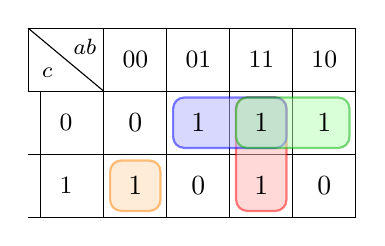
\begin{tikzpicture}[scale=0.8]
% Grid for cells
\draw (0,0) grid (4,2);

% Groupings (Uni)
% Group 1: ab=11, c=0,1 (Vertical)
\draw[rounded corners, fill=red!30, opacity=0.5, draw=red, thick] (2.1, 0.1) rectangle (2.9, 1.9);
% Group 2: c=0, ab=01,11 (Horizontal)
\draw[rounded corners, fill=blue!30, opacity=0.5, draw=blue, thick] (1.1, 1.1) rectangle (2.9, 1.9);
% Group 3: c=0, ab=11,10 (Horizontal)
\draw[rounded corners, fill=green!30, opacity=0.5, draw=green!70!black, thick] (2.1, 1.1) rectangle (3.9, 1.9);
% Group 4: c=1, ab=00 (Isolated)
\draw[rounded corners, fill=orange!30, opacity=0.5, draw=orange, thick] (0.1, 0.1) rectangle (0.9, 0.9);

% Values inside the map
\node at (0.5,1.5) {0}; \node at (1.5,1.5) {1}; \node at (2.5,1.5) {1}; \node at (3.5,1.5) {1};
\node at (0.5,0.5) {1}; \node at (1.5,0.5) {0}; \node at (2.5,0.5) {1}; \node at (3.5,0.5) {0};

% Headers
\draw (0,2) grid (4,3);
\node[font=\small] at (0.5,2.5) {00}; \node[font=\small] at (1.5,2.5) {01}; \node[font=\small] at (2.5,2.5) {11}; \node[font=\small] at (3.5,2.5) {10};
\draw (-1.2,0) grid (0,2);
\node[font=\small] at (-0.6,1.5) {0}; \node[font=\small] at (-0.6,0.5) {1};
\draw (-1.2,2) rectangle (0,3);
\draw (-1.2,3) -- (0,2);
\node[font=\footnotesize] at (-0.9, 2.3) {$c$};
\node[font=\footnotesize] at (-0.3, 2.7) {$ab$};
\end{tikzpicture}
\end{center}

\subsubsection*{Analisi dettagliata: Mintermini (Forma SOP)}
L'obiettivo della mappa è \textbf{semplificare una funzione logica} raggruppando gli \textbf{1}. La regola d'oro per trovare la formula di ogni blocco è: se una variabile \textbf{cambia valore} all'interno del gruppo \textbf{si elimina}. Se \textbf{rimane costante}, \textbf{si tiene} (normale se 1, negata se 0).

\begin{itemize}
    \item \textcolor{red}{\textbf{Il blocco ROSSO (verticale al centro):}} Le colonne ($ab$) sono sempre \textbf{11}, quindi $a=1$ e $b=1$ non cambiano e \textbf{le teniamo entrambe ($ab$)}. La riga ($c$) passa da 0 a 1, quindi cambia e \textbf{la eliminiamo}. Risultato: $\textcolor{red}{ab}$.
    \item \textcolor{blue}{\textbf{Il blocco BLU (orizzontale in alto a sinistra):}} La riga ($c$) è sempre \textbf{0}, quindi \textbf{la teniamo negata ($\overline{c}$)}. Le colonne ($ab$) passano da 01 a 11: la $a$ cambia (da 0 a 1) e si elimina, la $b$ resta 1 e si tiene. Risultato: $\textcolor{blue}{b\overline{c}}$.
    \item \textcolor{green!70!black}{\textbf{Il blocco VERDE (orizzontale in alto a destra):}} La riga ($c$) è sempre \textbf{0}, quindi \textbf{la teniamo negata ($\overline{c}$)}. Le colonne ($ab$) passano da 11 a 10: la $a$ resta 1 e si tiene, la $b$ cambia (da 1 a 0) e si elimina. Risultato: $\textcolor{green!70!black}{a\overline{c}}$.
    \item \textcolor{orange}{\textbf{Il blocco ARANCIO (cella isolata in basso):}} Non ha vicini, nessuna variabile cambia. Le teniamo tutte e tre per il valore che hanno: riga $c=1$, colonna $ab=00$. Risultato: $\textcolor{orange}{\overline{a}\,\overline{b}c}$.
\end{itemize}

Unendo tutti i risultati parziali con un segno \textbf{$+$} (OR), otteniamo:
\[ F = \textcolor{red}{ab} + \textcolor{blue}{b\overline{c}} + \textcolor{green!70!black}{a\overline{c}} + \textcolor{orange}{\overline{a}\,\overline{b}c} \]

\vspace{1.5em}

\begin{center}
\textbf{Semplificazione con Maxtermini (zeri)}\\[0.5em]
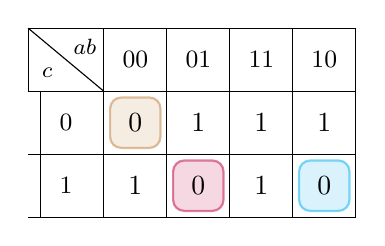
\begin{tikzpicture}[scale=0.8]
% Grid for cells
\draw (0,0) grid (4,2);

% Groupings (Zeri)
\draw[rounded corners, fill=purple!30, opacity=0.5, draw=purple, thick] (1.1, 0.1) rectangle (1.9, 0.9);
\draw[rounded corners, fill=cyan!30, opacity=0.5, draw=cyan, thick] (3.1, 0.1) rectangle (3.9, 0.9);
\draw[rounded corners, fill=brown!30, opacity=0.5, draw=brown, thick] (0.1, 1.1) rectangle (0.9, 1.9);

% Values inside the map
\node at (0.5,1.5) {0}; \node at (1.5,1.5) {1}; \node at (2.5,1.5) {1}; \node at (3.5,1.5) {1};
\node at (0.5,0.5) {1}; \node at (1.5,0.5) {0}; \node at (2.5,0.5) {1}; \node at (3.5,0.5) {0};

% Headers
\draw (0,2) grid (4,3);
\node[font=\small] at (0.5,2.5) {00}; \node[font=\small] at (1.5,2.5) {01}; \node[font=\small] at (2.5,2.5) {11}; \node[font=\small] at (3.5,2.5) {10};
\draw (-1.2,0) grid (0,2);
\node[font=\small] at (-0.6,1.5) {0}; \node[font=\small] at (-0.6,0.5) {1};
\draw (-1.2,2) rectangle (0,3);
\draw (-1.2,3) -- (0,2);
\node[font=\footnotesize] at (-0.9, 2.3) {$c$};
\node[font=\footnotesize] at (-0.3, 2.7) {$ab$};
\end{tikzpicture}
\end{center}

\subsubsection*{Analisi dettagliata: Maxtermini (Forma POS)}
Se con i mintermini cercavamo gli 1, qui ci concentriamo \textbf{solo sugli 0}. La logica si \textbf{ribalta completamente}: i valori si invertono (se vale 0 si scrive normale $a$, se vale 1 si scrive negata $\overline{a}$) e le operazioni si invertono (somme dentro le parentesi, moltiplicazioni fuori).

In questa mappa specifica, gli zeri si trovano in diagonale. Poiché non sono vicini in orizzontale o verticale, \textbf{sono isolati} e non possiamo raggrupparli. Li prendiamo uno per uno:

\begin{itemize}
    \item \textcolor{brown}{\textbf{Lo zero MARRONE (in alto a sinistra):}} Riga $c=0$, colonna $ab=00$ (quindi $a=0, b=0$). Applicando il ``mondo al contrario'', diventano tutti normali e li uniamo con il $+$. Risultato: $\textcolor{brown}{(a + b + c)}$.
    \item \textcolor{purple}{\textbf{Lo zero VIOLA (in basso al centro):}} Riga $c=1$, colonna $ab=01$ (quindi $a=0, b=1$). I valori a 1 si negano. Risultato: $\textcolor{purple}{(a + \overline{b} + \overline{c})}$.
    \item \textcolor{cyan}{\textbf{Lo zero AZZURRO (in basso a destra):}} Riga $c=1$, colonna $ab=10$ (quindi $a=1, b=0$). I valori a 1 si negano. Risultato: $\textcolor{cyan}{(\overline{a} + b + \overline{c})}$.
\end{itemize}

Moltiplichiamo (AND) tra loro i tre blocchi ottenuti per la soluzione finale:
\[ F = \textcolor{brown}{(a+b+c)} \cdot \textcolor{purple}{(a+\overline{b}+\overline{c})} \cdot \textcolor{cyan}{(\overline{a}+b+\overline{c})} \]

% ======================================================================
% mappe K a 4 variabili (sezione 4.2.2)
\subsection{Esempi di mappe di Karnaugh a 4 variabili}

\noindent Anche per 4 variabili si usa la codifica di Gray per disporre le combinazioni di due variabili ($ab$ e $cd$) sui lati della tabella. I raggruppamenti (implicanti) devono essere composti da un numero di ``1'' (o ``0'') pari a una potenza di due ($1, 2, 4, 8\ldots$) e formare rettangoli. Essi possono anche ``sconfinare'' da un bordo all'altro della mappa, poiché i bordi opposti sono adiacenti. 

L'obiettivo è coprire tutti gli 1 (o gli 0) col minor numero di raggruppamenti, il più larghi possibile. Analizziamo due funzioni diverse, tratte dagli appunti.

\begin{center}
\textbf{Mappa 1: Quando usare i Maxtermini NON conviene}\\[0.5em]
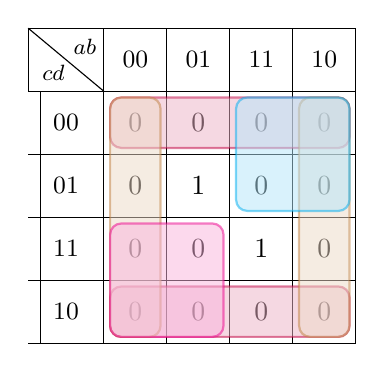
\begin{tikzpicture}[scale=0.8]
\draw (0,0) grid (4,4);
% Headers
\draw (0,4) grid (4,5);
\node[font=\small] at (0.5,4.5) {00}; \node[font=\small] at (1.5,4.5) {01}; \node[font=\small] at (2.5,4.5) {11}; \node[font=\small] at (3.5,4.5) {10};
\draw (-1.2,0) grid (0,4);
\node[font=\small] at (-0.6,3.5) {00}; \node[font=\small] at (-0.6,2.5) {01}; \node[font=\small] at (-0.6,1.5) {11}; \node[font=\small] at (-0.6,0.5) {10};
\draw (-1.2,4) rectangle (0,5); \draw (-1.2,5) -- (0,4);
\node[font=\footnotesize] at (-0.8, 4.3) {$cd$}; \node[font=\footnotesize] at (-0.3, 4.7) {$ab$};

% Values
\node at (0.5,3.5) {0}; \node at (1.5,3.5) {0}; \node at (2.5,3.5) {0}; \node at (3.5,3.5) {0};
\node at (0.5,2.5) {0}; \node at (1.5,2.5) {1}; \node at (2.5,2.5) {0}; \node at (3.5,2.5) {0};
\node at (0.5,1.5) {0}; \node at (1.5,1.5) {0}; \node at (2.5,1.5) {1}; \node at (3.5,1.5) {0};
\node at (0.5,0.5) {0}; \node at (1.5,0.5) {0}; \node at (2.5,0.5) {0}; \node at (3.5,0.5) {0};

% Groupings Maxterms
% (d) -> d=0 -> rows 00,10 -> (0,3)-(4,4) and (0,0)-(4,1)
\draw[rounded corners, fill=purple!30, opacity=0.5, draw=purple, thick] (0.1, 3.1) rectangle (3.9, 3.9);
\draw[rounded corners, fill=purple!30, opacity=0.5, draw=purple, thick] (0.1, 0.1) rectangle (3.9, 0.9);
% (b) -> b=0 -> cols 00,10 -> (0,0)-(1,4) and (3,0)-(4,4)
\draw[rounded corners, fill=brown!30, opacity=0.5, draw=brown, thick] (0.1, 0.1) rectangle (0.9, 3.9);
\draw[rounded corners, fill=brown!30, opacity=0.5, draw=brown, thick] (3.1, 0.1) rectangle (3.9, 3.9);
% (a'+c) -> a=1, c=0 -> cols 11,10 rows 00,01 -> (2,2)-(4,4)
\draw[rounded corners, fill=cyan!30, opacity=0.5, draw=cyan, thick] (2.1, 2.1) rectangle (3.9, 3.9);
% (a+c') -> a=0, c=1 -> cols 00,01 rows 11,10 -> (0,0)-(2,2)
\draw[rounded corners, fill=magenta!30, opacity=0.5, draw=magenta, thick] (0.1, 0.1) rectangle (1.9, 1.9);
\end{tikzpicture}
\end{center}

\subsubsection*{Analisi della Mappa 1: Perché i Maxtermini falliscono}
In questa prima funzione, abbiamo ben quattordici zeri e solo due uni. Se proviamo a usare i \textbf{Maxtermini} (raggruppando gli 0, logica inversa), l'alto numero di zeri ci costringe a fare ben \textbf{4 raggruppamenti} che si accavallano caoticamente sfruttando anche i bordi!
\begin{itemize}
    \item \textcolor{purple}{\textbf{Bordi orizzontali VIOLA (8 celle):}} Comprende le righe $cd=00,10$. Resta solo $d=0 \to d$. Risultato: $\textcolor{purple}{(d)}$.
    \item \textcolor{brown}{\textbf{Bordi verticali MARRONI (8 celle):}} Comprende le colonne $ab=00,10$. Resta solo $b=0 \to b$. Risultato: $\textcolor{brown}{(b)}$.
    \item \textcolor{cyan}{\textbf{Quadrato AZZURRO (4 celle, alto a dx):}} Colonne $11,10$ ($a=1 \to \overline{a}$) e righe $00,01$ ($c=0 \to c$). Risultato: $\textcolor{cyan}{(\overline{a}+c)}$.
    \item \textcolor{magenta}{\textbf{Quadrato MAGENTA (4 celle, basso a sx):}} Colonne $00,01$ ($a=0 \to a$) e righe $11,10$ ($c=1 \to \overline{c}$). Risultato: $\textcolor{magenta}{(a+\overline{c})}$.
\end{itemize}
Espressione trovata: $F = \textcolor{purple}{(d)} \cdot \textcolor{brown}{(b)} \cdot \textcolor{cyan}{(\overline{a}+c)} \cdot \textcolor{magenta}{(a+\overline{c})}$

Se invece usassimo i \textbf{Mintermini} per la stessa mappa, ci basterebbe raggruppare i due singoli \textbf{1} isolati (2 gruppi da una cella). Si otterrebbe $F = \overline{a}b\overline{c}d + abcd$ (solo \textbf{due} termini). \textbf{Conclusione:} con i maxtermini l'espressione si riduce, ma restano comunque molti termini (4 fattori, con raggruppamenti che si sovrappongono); con i mintermini bastano 2 termini, più facili da leggere e da realizzare. Conviene quindi usare i mintermini. In generale si sceglie la forma che richiede meno raggruppamenti.

\vspace{1.5em}

\begin{center}
\textbf{Mappa 2: Un buon uso dei Mintermini}\\[0.5em]
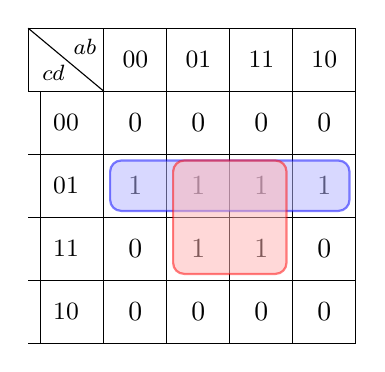
\begin{tikzpicture}[scale=0.8]
\draw (0,0) grid (4,4);
% Headers
\draw (0,4) grid (4,5);
\node[font=\small] at (0.5,4.5) {00}; \node[font=\small] at (1.5,4.5) {01}; \node[font=\small] at (2.5,4.5) {11}; \node[font=\small] at (3.5,4.5) {10};
\draw (-1.2,0) grid (0,4);
\node[font=\small] at (-0.6,3.5) {00}; \node[font=\small] at (-0.6,2.5) {01}; \node[font=\small] at (-0.6,1.5) {11}; \node[font=\small] at (-0.6,0.5) {10};
\draw (-1.2,4) rectangle (0,5); \draw (-1.2,5) -- (0,4);
\node[font=\footnotesize] at (-0.8, 4.3) {$cd$}; \node[font=\footnotesize] at (-0.3, 4.7) {$ab$};

% Values
\node at (0.5,3.5) {0}; \node at (1.5,3.5) {0}; \node at (2.5,3.5) {0}; \node at (3.5,3.5) {0};
\node at (0.5,2.5) {1}; \node at (1.5,2.5) {1}; \node at (2.5,2.5) {1}; \node at (3.5,2.5) {1};
\node at (0.5,1.5) {0}; \node at (1.5,1.5) {1}; \node at (2.5,1.5) {1}; \node at (3.5,1.5) {0};
\node at (0.5,0.5) {0}; \node at (1.5,0.5) {0}; \node at (2.5,0.5) {0}; \node at (3.5,0.5) {0};

% Groupings Minterms
\draw[rounded corners, fill=blue!30, opacity=0.5, draw=blue, thick] (0.1, 2.1) rectangle (3.9, 2.9);
\draw[rounded corners, fill=red!30, opacity=0.5, draw=red, thick] (1.1, 1.1) rectangle (2.9, 2.9);
\end{tikzpicture}
\end{center}

\subsubsection*{Analisi della Mappa 2 con i Mintermini}
In questa seconda funzione abbiamo meno uni (sei) che zeri (dieci). Ci conviene usare i \textbf{Mintermini} e raggruppare gli \textbf{1}:
\begin{itemize}
    \item \textcolor{blue}{\textbf{Rettangolo BLU (4 celle, riga intera):}} Copre tutta la riga $cd=01$. Quindi $c=0 \to \overline{c}$ e $d=1 \to d$. Le colonne variano tutte, quindi si eliminano $a$ e $b$. Risultato: $\textcolor{blue}{\overline{c}d}$.
    \item \textcolor{red}{\textbf{Quadrato ROSSO (4 celle, centrale):}} Copre le colonne $ab=01,11$ ($a$ cambia, resta $b=1 \to b$) e le righe $cd=01,11$ ($c$ cambia, resta $d=1 \to d$). Risultato: $\textcolor{red}{bd}$.
\end{itemize}
L'espressione ottimizzata risultante è semplicemente la somma dei due gruppi:
\[ F = \textcolor{blue}{\overline{c}d} + \textcolor{red}{bd} = (\overline{c}+b)d \]

% ======================================================================
\section{Codifica binaria}

Con $n$ bit posso descrivere $2^n$ valori in decimale.

\medskip
\begin{esercizio}{Esempio}$N = 13 \leftrightarrow 1101$.\end{esercizio}

\begin{definizione}{Conversione binario $\to$ decimale}
si moltiplica ogni cifra per la potenza di 2 corrispondente alla sua posizione e si somma:
\[
1101 \to 1\cdot2^3+1\cdot2^2+0\cdot2^1+1\cdot2^0 = 8+4+0+1=13
\]

\medskip
\textbf{Conversione decimale $\to$ binario}: si divide ripetutamente per 2, prendendo via via i resti dal basso verso l'alto:
\[
13 \to \frac{13}{2}=6\text{ resto }1 \to \frac{6}{2}=3\text{ resto }0 \to \frac{3}{2}=1\text{ resto }1 \to \frac{1}{2}=0\text{ resto }1
\]
\[
\Rightarrow 13 = 1101 \text{ (leggendo i resti dal basso verso l'alto)}
\]
\end{definizione}

\section{Codice BCD}

\begin{definizione}{BCD}
\textbf{BCD} (\emph{Binary Coded Decimal}): per scrivere le cifre decimali da 0 a 9 si usano 4 bit (3 bit sarebbero troppo pochi, dato che $2^3=8<10$).
\end{definizione}

\subsection{Esempio: display a 7 segmenti}

\begin{figure}[htpb]
    \centering
    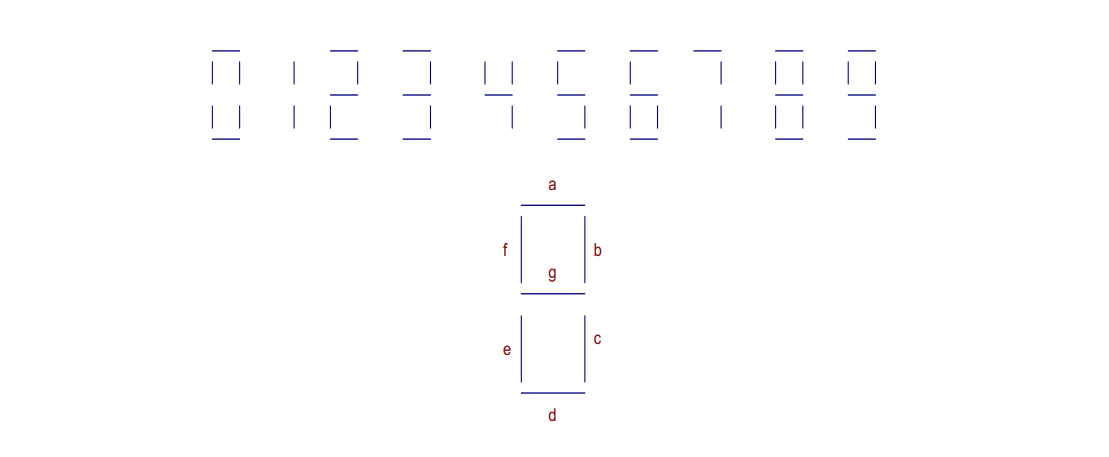
\includegraphics[width=0.4\linewidth]{7seg.png}
\end{figure}

\textit{Si vuole pilotare il segmento centrale ($g$) di un display a 7 segmenti a partire dalla cifra BCD in ingresso $a,b,c,d$. Il segmento centrale è spento solo per le cifre 0, 1 e 7.}

\medskip
\noindent Si costruisce la tabella di verità del segmento (con $a\leftrightarrow$ bit più significativo, $d\leftrightarrow$ bit meno significativo) e si segnano come \textbf{don't care} ($\times$) le combinazioni che non corrispondono a nessuna cifra BCD (cioè da 10 a 15), in modo da poter scegliere il loro valore così da semplificare il circuito:

\begin{center}
\begin{tabular}{cccc|c}
\toprule
$a$&$b$&$c$&$d$ & $g$\\
\midrule
0&0&0&0 & 0\\
0&0&0&1 & 0\\
0&0&1&0 & 1\\
0&0&1&1 & 1\\
0&1&0&0 & 1\\
0&1&0&1 & 1\\
0&1&1&0 & 1\\
0&1&1&1 & 0\\
1&0&0&0 & 1\\
1&0&0&1 & 1\\
\multicolumn{4}{c|}{1010 -- 1111} & $\times\;\times\;\times\;\times\;\times\;\times$\\
\bottomrule
\end{tabular}
\end{center}

\noindent La 2\textsuperscript{a} forma canonica (POS) del segmento, prima della semplificazione, contiene i tre maxtermini delle cifre 0, 1 e 7:
\[
F(a,b,c,d)=(a+b+c+d)\cdot(a+b+c+\overline{d})\cdot(a+\overline{b}+\overline{c}+\overline{d})
\]

\noindent Riportando la funzione (con i don't care) sulla mappa di Karnaugh a 4 variabili $cd\backslash ab$ e scegliendo opportunamente il valore dei don't care, si semplifica notevolmente il circuito:

\begin{center}
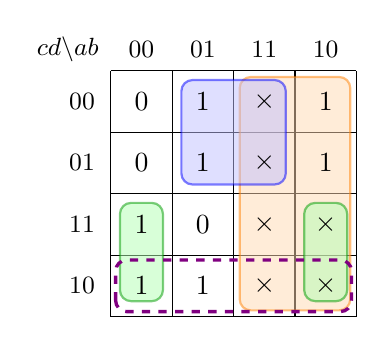
\begin{tikzpicture}[scale=0.78]
\draw (0,0) grid (4,4);
\node[font=\small] at (0.5,4.35) {00};
\node[font=\small] at (1.5,4.35) {01};
\node[font=\small] at (2.5,4.35) {11};
\node[font=\small] at (3.5,4.35) {10};
\node[font=\small, anchor=east] at (-0.1,3.5) {00};
\node[font=\small, anchor=east] at (-0.1,2.5) {01};
\node[font=\small, anchor=east] at (-0.1,1.5) {11};
\node[font=\small, anchor=east] at (-0.1,0.5) {10};
\node[font=\small] at (-0.7,4.35) {$cd{\backslash}ab$};
% raggruppamenti
\draw[rounded corners, fill=orange!30, opacity=0.5, draw=orange, thick] (2.1,0.1) rectangle (3.9,3.9);
\draw[rounded corners, fill=blue!25, opacity=0.5, draw=blue, thick] (1.15,2.15) rectangle (2.85,3.85);
\draw[rounded corners, fill=green!30, opacity=0.5, draw=green!60!black, thick] (0.15,0.25) rectangle (0.85,1.85);
\draw[rounded corners, fill=green!30, opacity=0.5, draw=green!60!black, thick] (3.15,0.25) rectangle (3.85,1.85);
\draw[rounded corners, draw=violet, very thick, dashed] (0.08,0.08) rectangle (3.92,0.92);
\node at (0.5,3.5) {0}; \node at (1.5,3.5) {1}; \node at (2.5,3.5) {$\times$}; \node at (3.5,3.5) {1};
\node at (0.5,2.5) {0}; \node at (1.5,2.5) {1}; \node at (2.5,2.5) {$\times$}; \node at (3.5,2.5) {1};
\node at (0.5,1.5) {1}; \node at (1.5,1.5) {0}; \node at (2.5,1.5) {$\times$}; \node at (3.5,1.5) {$\times$};
\node at (0.5,0.5) {1}; \node at (1.5,0.5) {1}; \node at (2.5,0.5) {$\times$}; \node at (3.5,0.5) {$\times$};
\end{tikzpicture}
\end{center}

\noindent Scegliendo i don't care in modo da formare i raggruppamenti più grandi possibile:
\begin{itemize}[leftmargin=1.5em, itemsep=1pt]
    \item \textcolor{orange}{\textbf{arancio}}: le colonne $ab=11$ e $ab=10$ (tutte 1 o don't care) danno $a$;
    \item \textcolor{blue}{\textbf{blu}}: colonne $01,11$ e righe $00,01$ danno $b\,\overline{c}$;
    \item \textcolor{green!60!black}{\textbf{verde}}: colonne $00$ e $10$ (adiacenti attraverso il bordo) e righe $11,10$ danno $\overline{b}\,c$;
    \item \textcolor{violet}{\textbf{viola}} (tratteggiato): la riga $cd=10$ dà $c\,\overline{d}$.
\end{itemize}
L'espressione semplificata diventa:
\[
a+c\overline{d}+\overline{b}c+b\overline{c} = a+c\overline{d}+(b\oplus c)
\]
molto più corta e immediata da realizzare rispetto alla forma canonica di partenza.

\begin{definizione}{Don't care}
I \textbf{don't care} si scelgono in modo da semplificare il più possibile il circuito risultante.
\end{definizione}

% ======================================================================
% circuito half adder — ingressi correttamente biforcati
\section{Sommatori}

\subsection{Semi-sommatore (half adder)}

\noindent Un \textbf{semi-sommatore} (half adder) è un circuito combinatorio in grado di eseguire la somma di due singoli bit ($a_i$ e $b_i$). Esso produce due uscite: il bit di somma $\Sigma_i$ e il bit di riporto generato $C_{i+1}$ (carry out). L'equazione logica che descrive la somma è un'operazione XOR ($\Sigma_i = a_i \oplus b_i$), mentre il riporto è dato da un'operazione AND ($C_{i+1} = a_i \cdot b_i$). 
Il limite del semi-sommatore è che non prevede un ingresso per il riporto proveniente da uno stadio precedente, limitandone l'utilizzo al solo bit meno significativo di un'addizione su più bit.

\begin{center}
\begin{circuitikz}[scale=1.0, every node/.style={scale=1.0}]
% Porte
\node[xor port] (XH) at (0, 1.5) {};
\node[and port] (AH) at (0, 0) {};

% Nodi di ingresso (allineati dinamicamente alle porte per evitare linee storte)
\coordinate (Ain) at (-2.5, 0 |- XH.in 1);
\coordinate (Bin) at (-2.5, 0 |- XH.in 2);
\node[left] at (Ain) {$a_i$};
\node[left] at (Bin) {$b_i$};

% Connessioni principali
\draw (Ain) -- (XH.in 1);
\draw (Bin) -- (XH.in 2);

% Derivazioni (i pallini sono centrati dinamicamente sulla linea)
\coordinate (Atap) at (-1.8, 0 |- XH.in 1);
\coordinate (Btap) at (-1.1, 0 |- XH.in 2);

\draw (Atap) to[short, *-] (Atap |- AH.in 1) -- (AH.in 1);
\draw (Btap) to[short, *-] (Btap |- AH.in 2) -- (AH.in 2);

% Uscite
\draw (XH.out) -- ++(0.7,0) node[right]{$\Sigma_i$};
\draw (AH.out) -- ++(0.7,0) node[right]{$C_{i+1}$};

\end{circuitikz}
\end{center}

\noindent Tabella di verità del semi-sommatore:

\begin{center}
\begin{tabular}{cc|cc}
\toprule
$a_i$ & $b_i$ & $\Sigma_i$ & $C_{i+1}$\\
\midrule
0&0&0&0\\
0&1&1&0\\
1&0&1&0\\
1&1&0&1\\
\bottomrule
\end{tabular}
\end{center}

\subsection{Sommatore completo (full adder)}

\noindent Il \textbf{sommatore completo} (full adder) risolve il limite del semi-sommatore aggiungendo un terzo ingresso $C_i$ per il riporto proveniente da uno stadio precedente. L'uscita somma $\Sigma_i$ vale 1 se il numero di ingressi a 1 è dispari, mentre il riporto $C_{i+1}$ vale 1 se almeno due ingressi sono a 1.
\medskip

\noindent Il circuito può essere ottenuto combinando due semi-sommatori e una porta OR finale per i riporti, in modo da tenere conto di tutti gli addendi:

\begin{center}
\begin{circuitikz}[scale=1.0, every node/.style={scale=1.0}]
% Primo HA
\draw (0, 0.3) rectangle (2.5, 2.3);
\node at (1.25, 1.3) {HA 1};
\node[right] at (0, 1.8) {$a_i$};
\node[right] at (0, 0.8) {$b_i$};
\node[left] at (2.5, 1.8) {$\Sigma'_i$};
\node[left] at (2.5, 0.8) {$C'_i$};

% Secondo HA
\draw (4.5, 1.3) rectangle (7.0, 3.3);
\node at (5.75, 2.3) {HA 2};
\node[right] at (4.5, 2.8) {$C_i$};
\node[right] at (4.5, 1.8) {$\Sigma'_i$};
\node[left] at (7.0, 2.8) {$\Sigma_i$};
\node[left] at (7.0, 1.8) {$C''_i$};

% OR gate
\node[or port] (OR) at (9.5, 1.3) {};

% Connessioni primo HA
\draw (-1.5, 1.8) node[left] {$a_i$} -- (0, 1.8);
\draw (-1.5, 0.8) node[left] {$b_i$} -- (0, 0.8);

% Connessioni intermedie e Cin
\draw (2.5, 1.8) -- (4.5, 1.8); % Linea dritta, nessun gradino!
\draw (-1.5, 2.8) node[left] {$C_i$} -- (4.5, 2.8); % Linea dritta, nessun gradino!

% Connessioni Carry
\draw (2.5, 0.8) -- (8.2, 0.8) |- (OR.in 2);
\draw (7.0, 1.8) -- (8.2, 1.8) |- (OR.in 1);

% Uscite finali
\draw (7.0, 2.8) -- (10.5, 2.8) node[right] {$\Sigma_i$};
\draw (OR.out) -- (10.5, 1.3) node[right] {$C_{i+1}$};

\end{circuitikz}
\end{center}

\noindent Tabella di verità del sommatore completo (con $\Sigma_i'$, $C_{i+1}'$ uscite del primo HA):

\begin{center}
\begin{tabular}{ccc|ccc}
\toprule
$a_i$ & $b_i$ & $C_i$ & $\Sigma_i'$ & $\Sigma_i$ & $C_{i+1}$\\
\midrule
0&0&0&0&0&0\\
0&0&1&0&1&0\\
0&1&0&1&1&0\\
0&1&1&1&0&1\\
1&0&0&1&1&0\\
1&0&1&1&0&1\\
1&1&0&0&0&1\\
1&1&1&0&1&1\\
\bottomrule
\end{tabular}
\end{center}

\subsubsection*{Logica dietro la tabella di verità}

Le due uscite del full adder obbediscono a regole semplici che si ricavano direttamente dal significato fisico della somma binaria.

\begin{itemize}
    \item \textbf{Bit di somma $\Sigma_i$ — ``parità'' degli ingressi:}
    $\Sigma_i = 1$ ogni volta che il numero totale di ingressi a \textbf{1} è \emph{dispari} (uno solo oppure tutti e tre). Questo coincide esattamente con l'\textbf{XOR a tre vie}:
    \[
        \Sigma_i = a_i \oplus b_i \oplus C_i
    \]
    Si può verificare intuitivamente: $1+1+0 = 2_{10} = 10_2$, la cifra delle unità è \textbf{0}; $1+1+1 = 3_{10} = 11_2$, la cifra delle unità è \textbf{1}. In entrambi i casi conta solo la parità degli addendi.

    \item \textbf{Bit di riporto $C_{i+1}$ — ``maggioranza'' degli ingressi:}
    $C_{i+1} = 1$ ogni volta che \emph{almeno due} ingressi su tre sono a \textbf{1} (funzione di maggioranza). Algebricamente:
    \[
        C_{i+1} = a_i b_i + b_i C_i + a_i C_i
    \]
    Ogni termine rappresenta una coppia che, sommata, produce riporto ($1+1 \ge 2$).
\end{itemize}

Queste due formule — e quindi l'intera tabella — si ricavano senza dover enumerare tutti gli 8 casi: basta ricordare che $\Sigma_i$ conta la \emph{parità} e $C_{i+1}$ la \emph{maggioranza} dei tre bit in ingresso.

% ======================================================================
\section*{Riepilogo del Capitolo}

\begin{important}
Dagli assiomi di Boole (Huntington) derivano il \textbf{teorema di semplificazione} e le \textbf{leggi di De Morgan}, che permettono di passare da una tabella di verità alle forme canoniche SOP/POS e di minimizzarle con le \textbf{mappe di Karnaugh}, realizzabili con le porte universali NAND/NOR.
\end{important}

\begin{note}
\textbf{Formule fondamentali:}
\begin{itemize}
    \item \textbf{Leggi di De Morgan:} $\overline{x+y+\cdots} = \overline{x}\cdot\overline{y}\cdots$; $\;\overline{x\cdot y \cdots} = \overline{x}+\overline{y}+\cdots$.
    \item \textbf{Teorema di semplificazione:} $xy+x\overline{y}=x$ (duale: $(x+y)(x+\overline{y})=x$).
    \item \textbf{Porte universali:} NAND e NOR realizzano da sole NOT, AND, OR, XOR (insieme funzionalmente completo).
    \item \textbf{Mappe di Karnaugh:} righe/colonne ordinate in codice Gray (\cref{ch:gray-ascii}), così che celle adiacenti differiscano di un solo bit; si raggruppano potenze di 2 di $1$ (SOP) o di $0$ (POS).
    \item \textbf{Full Adder:} $\Sigma_i = a_i\oplus b_i\oplus C_i$ (parità), $\; C_{i+1}=a_ib_i+b_iC_i+a_iC_i$ (maggioranza).
\end{itemize}
\end{note}

